 
TThe given equation is of the form
\begin{align}
   \vec{x}^T\vec{V}\vec{x}+f=0
\end{align}
The matrix $\vec{V}$ can be decomposed as
\begin{align}
    \vec{V}=\vec{P}\vec{D}\vec{P}^T\label{eq:solutions/3/4/10/2}\\
    \text{where  }\vec{D}=\myvec{\lambda_1&0\\0&\lambda_2}
\end{align}
$\lambda_1$ and $\lambda_2$ are Eigen values of $\vec{V}$ , and
$\vec{P}$ contains the Eigen vectors corresponding to the Eigen values $\lambda_1$ and $\lambda_2$
\begin{align}
\vec{x}=\vec{P}\vec{y}+\vec{c}
\end{align}
indicates the linear transformation where $\vec{P}$ indicates the rotation of axes and $\vec{c}$ gives the shift of origin.
\begin{align}
  \vec{V}=\myvec{41&12\\12&34}\\
  det(\vec{V} )=\mydet{41&12\\12&34}>0
\end{align}
So,the given equation represents an ellipse\\
To find the Eigen values of $\vec{V}$
\begin{align}
    \mydet{\lambda\vec{I}-\vec{v}}=0\\
    \implies \mydet{\lambda-41&-12\\-12&\lambda-34}=0\\
    \implies \lambda^2-75\lambda+1250=0\\
    \implies \lambda_1=50,\lambda_2=25\\
    \vec{D}=\myvec{50&0\\0&25}
\end{align}
Finding Eigen vector $\vec{p}_1$ ,
\begin{align}
\lambda_1\vec{I}-\vec{V}= \myvec{9&-12\\-12&16}\xleftrightarrow[R_2\leftarrow R_2/4]{R_1\leftarrow R_1/3}\myvec{3&-4\\-3&4}\\
\xleftrightarrow[]{R_2\leftarrow R_1+R_2}\myvec{3&-4\\0&0}\\
\implies \vec{p_1}=\frac{1}{\sqrt{4^2+3^2}}\myvec{4\\3}=\myvec{\frac{4}{5}\\\frac{3}{5}}
\end{align}
Similarly,
\begin{align}
  \lambda_2\vec{I}-\vec{V}= \myvec{-16&-12\\-12&-9}\xleftrightarrow[R_2\leftarrow R_2/-3]{R_1\leftarrow R_1/-4}\myvec{4&3\\4&3}\\
\xleftrightarrow[]{R_2\leftarrow R_1-R_2}\myvec{4&3\\0&0}\\
\implies \vec{p_2}=\frac{1}{\sqrt{4^2+3^2}}\myvec{-3\\4}=\myvec{\frac{-3}{5}\\\frac{4}{5}}\\\text{ Therefore, } \vec{P}=\myvec{\vec{p_1}&\vec{p_2}}=\myvec{\frac{4}{5}&\frac{-3}{5}\\ \frac{3}{5}&\frac{4}{5}}
\end{align}
From \eqref{eq:solutions/3/4/10/2} $\vec{V}$ can be rewritten as
\begin{align}
    \vec{V}=\myvec{\frac{4}{5}&\frac{-3}{5}\\ \frac{3}{5}&\frac{4}{5}}\myvec{50&0\\0&25}\myvec{\frac{4}{5}&\frac{3}{5}\\ \frac{-3}{5}&\frac{4}{5}}
\end{align}
\eqref{eq:solutions/3/4/10/1} can be now rewritten as
\begin{align}
25\left[\vec{x}^T\myvec{\frac{4}{5}&\frac{-3}{5}\\ \frac{3}{5}&\frac{4}{5}}\myvec{2&0\\0&1}\myvec{\frac{4}{5}&\frac{3}{5}\\ \frac{-3}{5}&\frac{4}{5}}\vec{x}\right]=75\\
  \left[\myvec{\frac{4}{5}&\frac{3}{5}\\ \frac{-3}{5}&\frac{4}{5}}\vec{x}\right]^T\myvec{2&0\\0&1}\left[\myvec{\frac{4}{5}&\frac{3}{5}\\ \frac{-3}{5}&\frac{4}{5}}\vec{x}\right]= 3\label{eq:solutions/3/4/10/3}
\end{align}
 Consider the rotation transformation 
\begin{align}
  \vec{x}=\vec{P}\vec{y}\\
  \implies \vec{x}=\myvec{\frac{4}{5}&\frac{-3}{5}\\ \frac{3}{5}&\frac{4}{5}}\vec{y}\label{eq:solutions/3/4/10/4}\\
  \vec{P}^{-1}\vec{x}=\vec{P}^{-1}\vec{P}\vec{y}\\
  \implies \vec{y}= \vec{P}^{-1}\vec{x}\\
  \text{But, }\vec{P}^{-1}=\vec{P}^T\\
  \implies \vec{y}=\myvec{\frac{4}{5}&\frac{3}{5}\\ \frac{-3}{5}&\frac{4}{5}}\vec{x}
\end{align}

Using \eqref{eq:solutions/3/4/10/4} in \eqref{eq:solutions/3/4/10/3}, the ellipse equation can be rewritten as
\begin{align}
     \vec{y}^T\myvec{2&0\\0&1}\vec{y}=3
\end{align}
\begin{figure}[!ht]
\centering
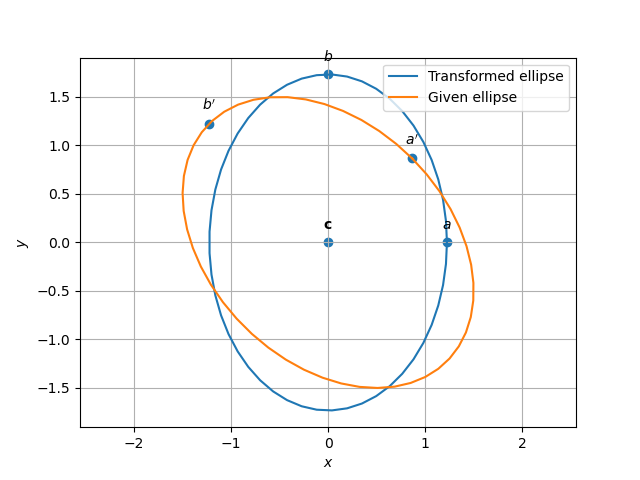
\includegraphics[width=\columnwidth]{./solutions/3/4/10/plot.png}
\caption{plot showing the original and rotated ellipse}
\label{eq:solutions/3/4/10/Fig}
\end{figure}


